\documentclass{tufte-handout}
\pagenumbering{arabic}
\usepackage{amsmath}
\usepackage[pdftex]{graphicx}
\usepackage{color}
\usepackage{enumitem}
\usepackage{natbib}
\usepackage{comment}
\usepackage{bm}
\usepackage{mdwlist}

% The following package makes prettier tables.  We're all about the bling!
\usepackage{booktabs}

% The units package provides nice, non-stacked fractions and better spacing
% for units.
\usepackage{units}

\newcommand{\angstrom}{\text{\normalfont\AA}}

% The fancyvrb package lets us customize the formatting of verbatim
% environments.  We use a slightly smaller font.
\usepackage{fancyvrb}
\fvset{fontsize=\normalsize}

% Small sections of multiple columns
\usepackage{multicol}

\usepackage{hyperref}
\hypersetup{
    colorlinks=true,       % false: boxed links; true: colored links
    linkcolor=red,       % color of internal links
    citecolor=red,        % color of links to bibliography
    filecolor=magenta,      % color of file links
    urlcolor=blue           % color of external links
}

\newcommand{\cs}{${}^{137}_{\ 55}{\rm Cs}$ }
\newcommand{\ba}{${}^{137}_{\ 56}{\rm Ba }$}
\newcommand{\bam}{${}^{137}_{\ 56}{\rm Ba^* }$}

%\pagestyle{myheadings}
%\markright{Fall~2016\hspace{1.9in}Mechanics Lab}


%\documentclass[12pt]{aastex}
%\usepackage{graphicx,mdwlist,longtable,url}
%\usepackage[final]{pdfpages}
%
%\usepackage[title,titletoc,toc]{appendix}
%\usepackage{longtable}
%
%% left-justify the section headings and make them bigger
%\usepackage{titlesec}
%\newcommand*{\justifyheading}{\raggedright}
%\titleformat*{\section}{\Large\bfseries}
%\titleformat*{\subsection}{\large\bfseries}
%
%\renewcommand{\bottomfraction}{0.9}
%
%\setlength{\parindent}{0.cm}
%\setlength{\parskip}{0.3cm}
%\setlength{\topmargin}{-1.3cm}
%\setlength{\textheight}{9in}
%\setlength{\evensidemargin}{0cm}
%\setlength{\textwidth}{6.46in}
%\setlength{\oddsidemargin}{0in}
%
%\pagestyle{myheadings}
%\markright{Fall~2016\hspace{1.9in}Mechanics Lab}
%
%% these make the longtables span the width of \textwidth
%\setlength\LTleft{0pt}
%\setlength\LTright{0pt}



\begin{document}
{\LARGE {\em 
\noindent Modern Physics---PHYS~220
\vspace{0.5mm}

\noindent Fall 2023
\vspace{3mm}
}}


{\LARGE {\em \noindent Lab: The Speed of Light}}

\large{\noindent Josh Diamond,  John Cummings, George Hassel, Mark Rosenberry, \& Matt Bellis}


\vspace{0.5cm}
\noindent{\bf \LARGE Week 2}\\
\vspace{0.5cm}


\section{Overview}

In this lab you will perform an updated version of the experiment Galileo
described in {\em Discourses and Mathematical Demonstrations Relating to Two New
  Sciences} to measure the speed of light.  Although the inherent uncertainties
of this technique are reduced in this version by using modern technology, the
principle of the measurement is the same: determine the time required for light
to traverse an known distance and calculate the velocity using
\[
v=\frac{\Delta x}{\Delta t}
\]


\section{Theory}

The velocity of light in free space is an important and intriguing 
constant of nature. Whether the light comes from a laser on a desktop 
or from a star that is hurling away at fantastic speeds, the velocity of 
light will yield the same constant value. In more precise terminology, 
the velocity of light is independent of the relative velocities of the light 
source and the observer. 

As Einstein first presented in his Special Theory of Relativity, the 
speed of light is critically important in some surprising ways: 
\begin{enumerate}
\item The velocity of light establishes an upper limit to the velocity that 
may be imparted to any object.
\item Objects moving near the velocity of light follow a set of physical 
laws drastically different, not only from Newton's Laws, but from 
the basic assumptions of human intuition.
\end{enumerate}

It is not surprising that a great deal of time and effort has been invested 
in measuring the speed of light. Some of the most accurate 
measurements were made by Albert Michelson between 1926 and 
1929. Michelson measured the velocity of light in air to be $2.99712\times10^8$~m/s. From this result, he deduced the velocity in free space to be $2.99796 \times 10^8$~m/s.

It is interesting to note that the ``ultimate speed limit,'' $c$, is the speed of light in the vacuum.  Material objects can, and indeed do, go faster that the speed of light in media such as air with no violation of special relativity or ``strange'' effects such as time travel or breakdown in causality.  If the object is charged, such as an electron, we do observe some interesting phenomena such as Cherenkov radiation.
 Cherenkov radiation is an electromagnetic analog of a sonic boom.  The blue glow that surrounds the underwater fuel rods in a reactor core is Cherenkov light, due to high energy electrons emitted by the fuel rods traveling faster than light in the water.

\begin{figure}
\centering
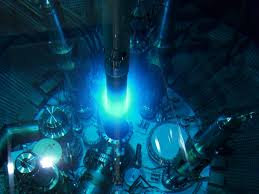
\includegraphics{../images/cherenkov.jpg}
\caption{Photograph of the FRM II research reactor near Munich, Germany}
\end{figure}


%\vspace{1cm}
In this experiment, you will measure the speed of light using a laser 
modulated at a very high frequency and an oscilloscope. You will 
measure the time, $\Delta t$, that elapses while the light signal travels a 
known distance, $\Delta d$, and you will calculate the speed of light, which is 
defined as 
\[
v = \frac{\Delta d}{\Delta t}
\]. 

The light signal, originating at the laser, will travel to the mirror and 
back to the light receiver. You will vary $\Delta d$ by moving the mirror and 
measuring the corresponding effect on $\Delta t$ with the oscilloscope.
It is not necessary (or practical) to measure the actual elapsed time, 
since we are only interested in how $\Delta t$ changes as $\Delta d$ varies. 
Therefore, you will actually measure an elapsed time $\Delta t^\prime$ relative to an 
arbitrary (but constant) baseline. This elapsed time can be expressed 
mathematically as:
\begin{equation}
\label{eq1}
\Delta t^\prime = \Delta t + t_k
\end{equation}
where $t_k$ is an unknown constant. For the same reason, you can also 
measure $\Delta d^\prime$ instead of $\Delta d$ where
\begin{equation}
\label{eq2}
\Delta d^\prime = \Delta d + d_k
\end{equation}
The equation of a line fitted to a plot of $\Delta d^\prime$ vs.\ $\Delta t^\prime$ is 
\begin{equation}
\label{eq3}
\Delta d^\prime = m \Delta t^\prime
\end{equation}
where $m$ represents the slope of the line. The combinations of 
equations \ref{eq1}, \ref{eq2}, and \ref{eq3} yields
\begin{align}
\label{eq4}
\Delta d & = m \Delta t + \left( m t_k - d_k \right) \nonumber \\
               & = m \Delta t + b 
\end{align}
where b is another arbitrary constant. In equation~\ref{eq4}, it is evident that 
the slope, $m$, equals $\Delta d/\Delta t$, which is the speed of light in air.

\section{Notes on Equipment}

The laser used in this experiment is a diode laser, which allows us to easily turn it on and off quickly; 3 MHz in this experiment.  This laser is a Class 2 laser, meaning its power is less than 1mW and the blink reflex should limit exposure to safe levels.  Intentionally suppressing the blink reflex could lead to permanent eye damage, and in any event, you should never look directly into the laser beam or shine it in anyone's eye.  If you are having trouble seeing the beam for alignment, a useful trick is to insert a piece of paper in the beam to locate the beam spot.

\begin{figure}
\centering
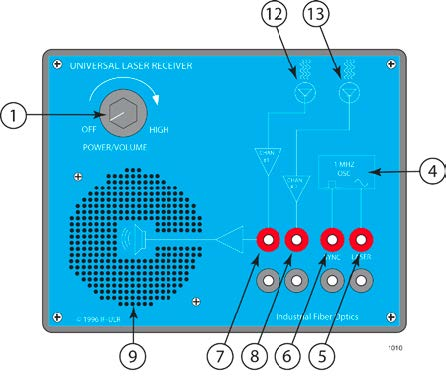
\includegraphics{../images/if-lsl-sa1opman-revd.jpg}
\caption{Universal Laser Receiver, top view.}
\label{ULRtop}
\end{figure}

\begin{figure}
\centering
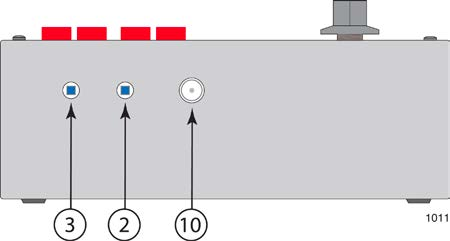
\includegraphics{../images/if-lsl-sa1opman-revdfront.jpg}
\caption{Universal Laser Receiver, front view.}
\label{ULRfront}
\end{figure}

The light receiver used in this experiment was designed for receiving both audio and video signals encoded and transmitted using modulated light.  There are two detectors in the receiver box, and you should see two windows for the sensitive elements (\#'s 12 or 13 in Fig. \ref{ULRtop} or \#'s 2 or 3 in Fig. \ref{ULRfront}).
%We will be using the video  element in this experiment, make sure you focus the light onto the correct element and the switch is set to the ``Video'' position.
Either the Channel 1 or Channel 2 detector should be suitable for this experiment.  Note which element you focus the light onto, and be sure to connect the banana plugs to the corresponding jacks (\#'s 7 or 8 in Fig. \ref{ULRtop}).   

The concave mirror helps focus the light after it is reflected.  Adjusting screws are useful to re-aim the reflected beam, and are often the only adjustment necessary.  The mirror is a sensitive optical element, please do not touch the front surface or drop the mirror.

\begin{figure}
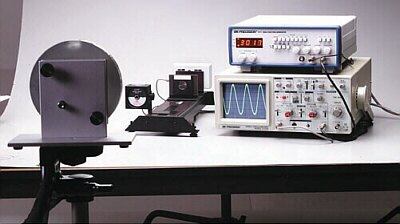
\includegraphics{../images/AP8586.jpg}
\caption{Example set up of apparatus.}
\end{figure}

\section{Procedures}

In this lab you will produce a {\em modulated} beam of laser light using the diode laser.  This modulation involves turning the diode on and off very rapidly (several million times a second) using a function generator.  A signal from a function generator with a frequency near 3 MHz will drive the laser diode.  The light produced by this laser will be reflected from a mirror and made to fall on a sensitive, fast light detector which produces a voltage proportional to the intensity of the light falling on it.  By observing the two signals (the signal modulating the diode and the output of the light detector) with an oscilloscope, you can measure the time delay caused by the travel time of the light signal.  You will measure this travel time for various distances by moving the mirror.

\subsection{Set up}

\begin{enumerate}
\item If the laser is not already on its L-shaped bracket, mount it with the
bracket bent away from the laser (Figure~\ref{fig:laser}).
\begin{figure}[h]
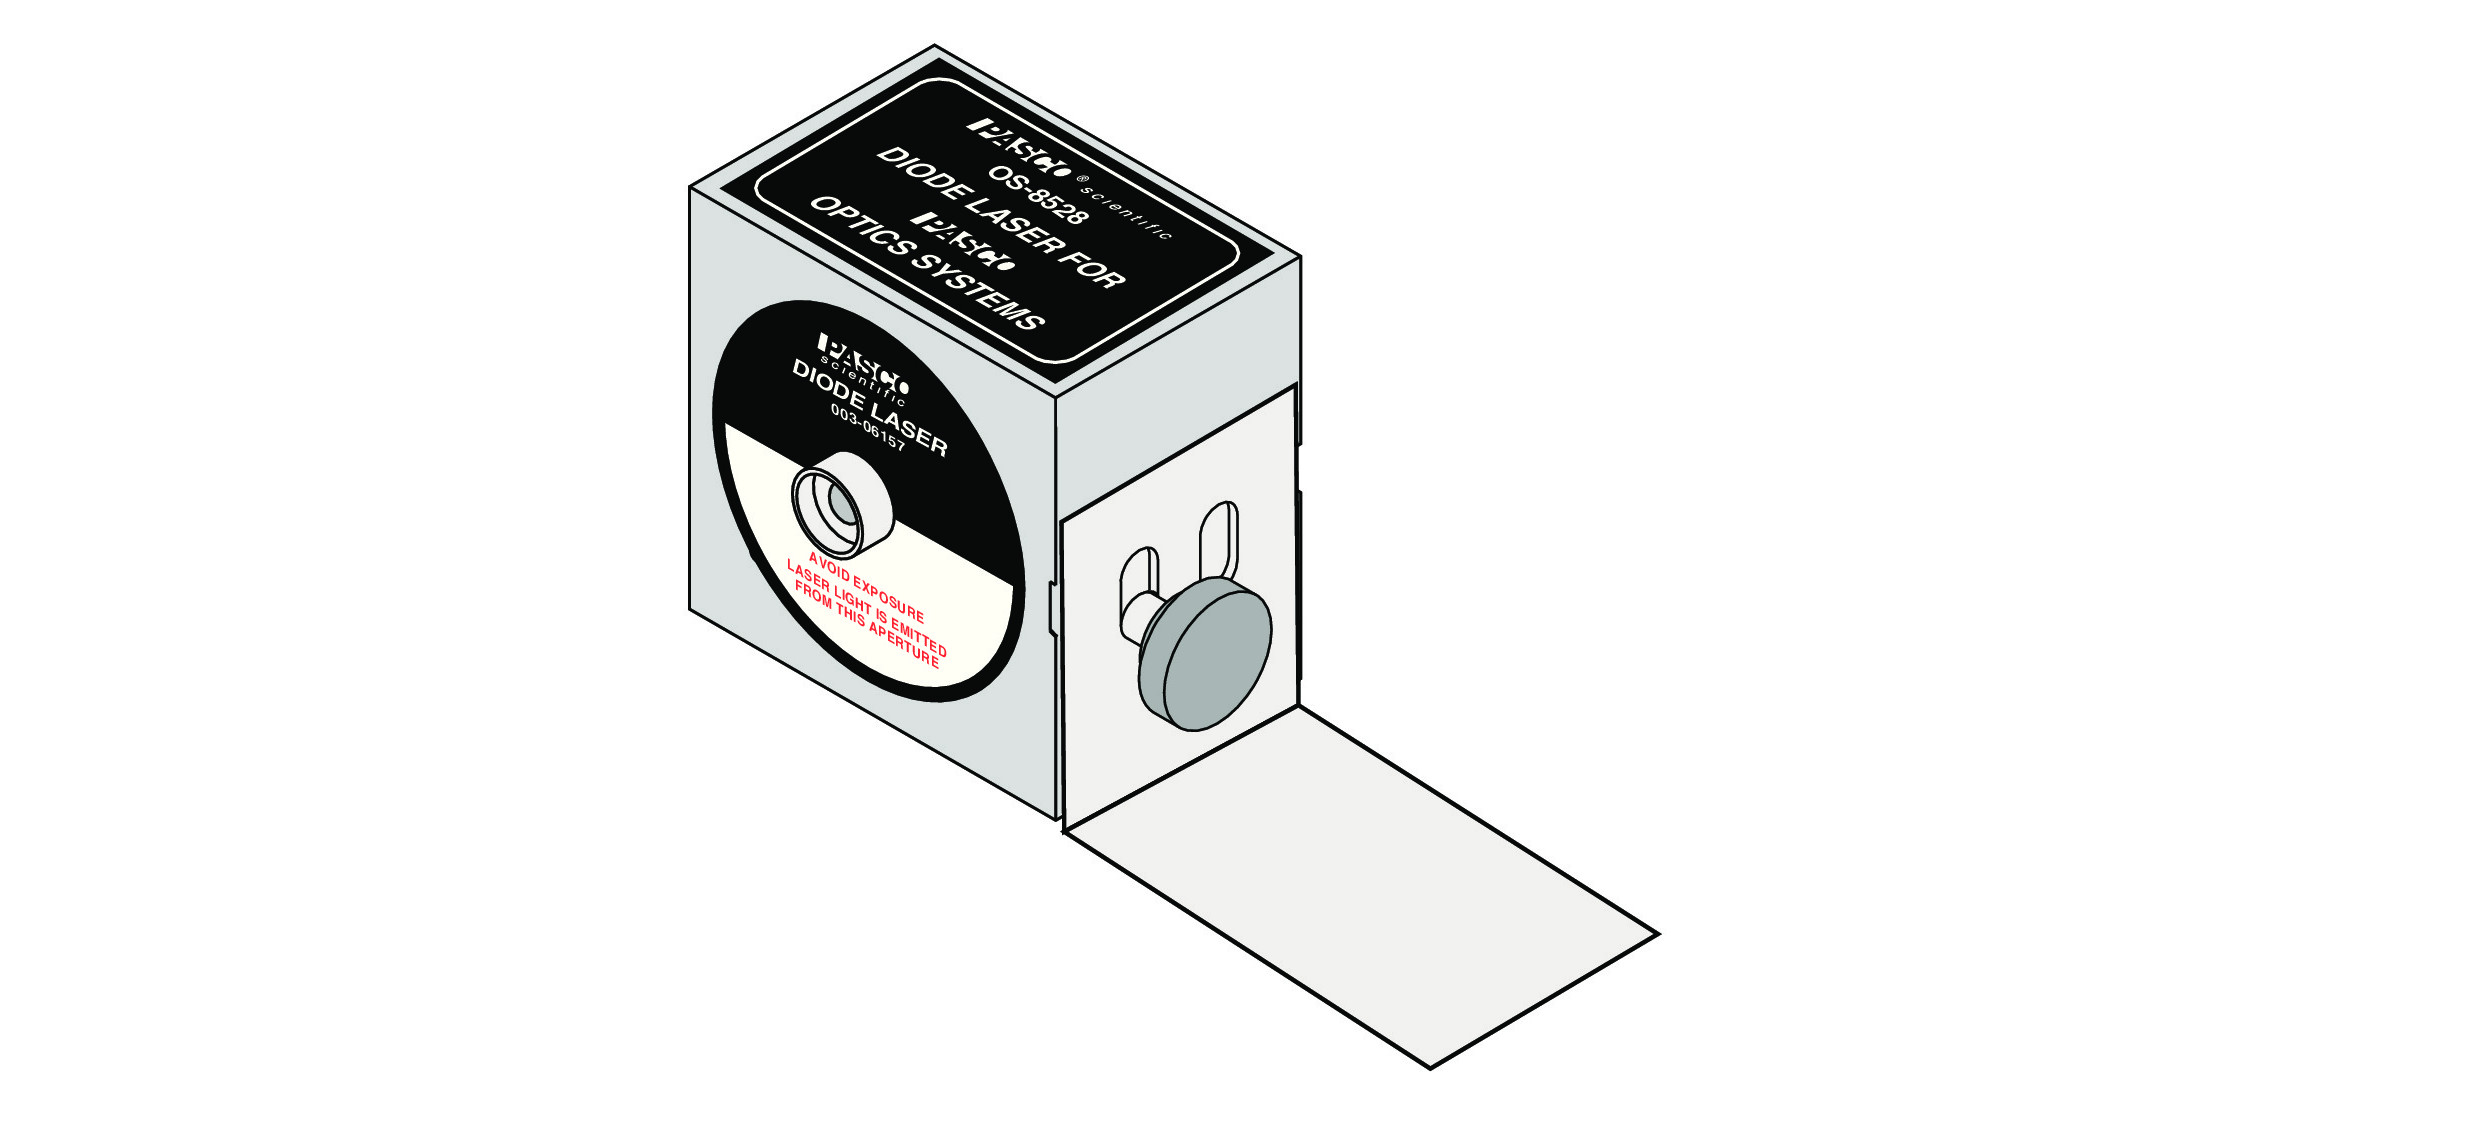
\includegraphics{../images/diode-laser.jpg}
\caption{\label{fig:laser} Laser with bracket}
\end{figure}

\item Place the alignment bench on a horizontal surface. Working on the floor in the hallway is probably easiest.  You will need 
10 to 20 m of clear space in front of the laser.  Place the mirror a few meters in front of the laser.

%5. Mount the mirror on the tripod and place it a few meters in front of 
%the laser. Adjust the tripod so that the mirror is at the same height 
%as the laser. (see Figure 3 for the setup.)

\item Arrange the laser, lens, receiver and two component carriers on the
laser alignment bench (Figure~\ref{fig:align}).
\begin{figure}[h]
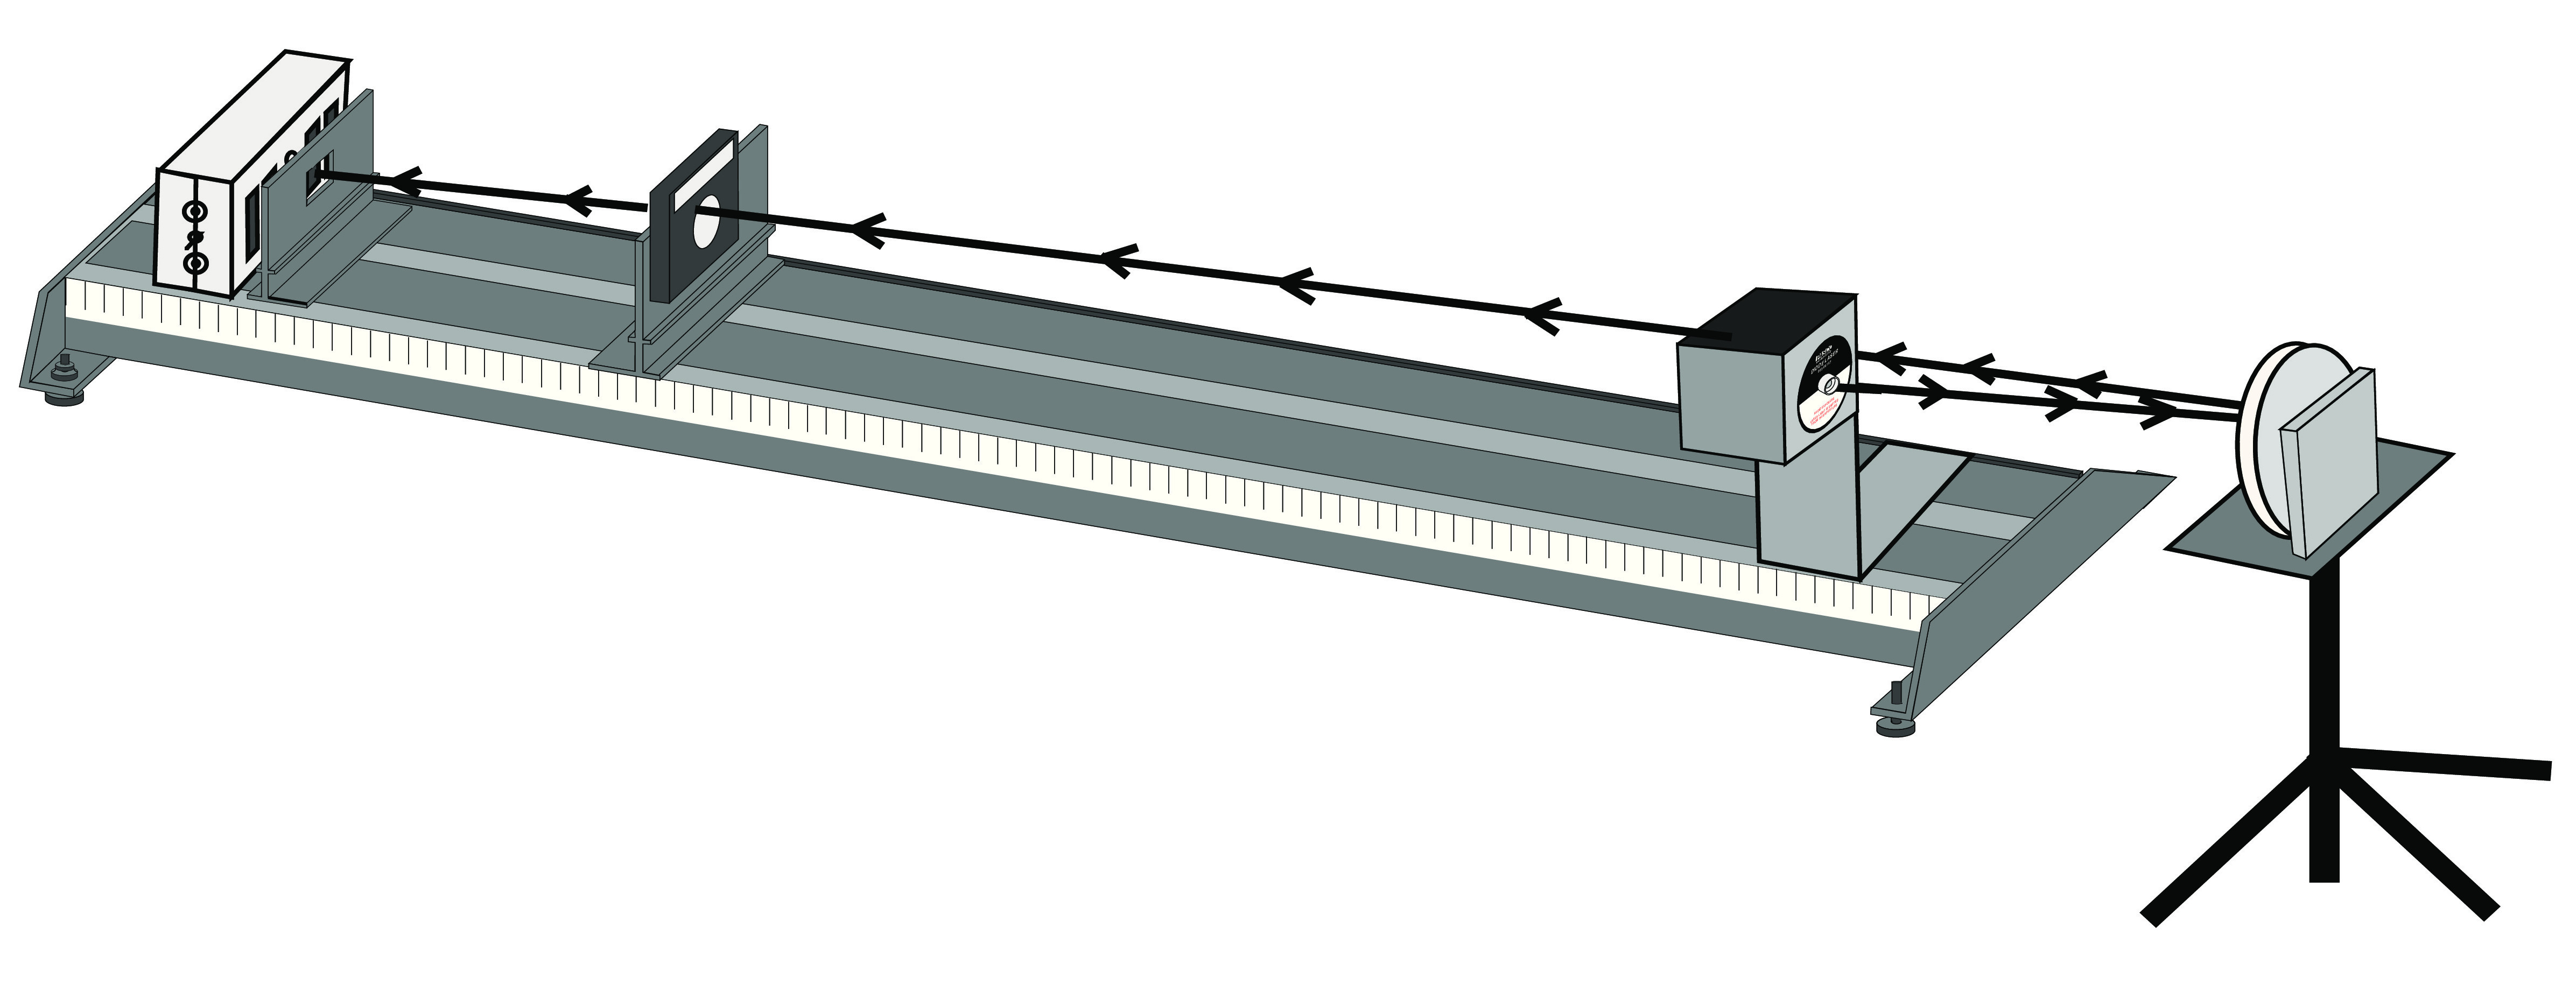
\includegraphics{../images/aligning.jpg}
\caption{\label{fig:align} Aligning the lens, carriers, and receiver with the laser }
\end{figure}
% this may work better without the lens.  at least it is much easier to align.

%6. Mark the position of the mirror on the floor with tape. (Attach a 
%plumb bob to the tripod, so that you mark a point directly below the 
%mirror.

\item Mark the position of the mirror on the floor with tape.  With tape, mark the floor at regular intervals to about 10-20 meters 
from the laser. Allow for at least 10 different intervals within the 
allotted space. 

\item Cable the system:
\begin{itemize}
\item connect the TTL output of the function generator to channel 1 of the oscilloscope.  
\item connect the  output (\# 7 or 8 of Fig. \ref{ULRtop})  of the laser receiver to channel 2 of the oscilloscope.
\item connect the power jack of the laser to the output of the function generator.
\item connect the ``wall wart'' power supply to the laser detector.
\end{itemize}

%8. Using the BNC male-to-male cable, connect the TTL output of the 
%function generator to channel 1 of the oscilloscope.

%9. Using the RCA male-to-BNC male cable, connect the “Video” 
%output of the receiver to channel 2 of the oscilloscope.

%10. Using the phone plug-to-BNC male cable, connect the power jack 
%of the laser to the output of the function generator.

\item Set the function generator for a square wave, and turn on the DC 
Offset. Turn the Output and DC Offset knobs all the way down.

\item Turn the laser switch to the ``on'' position and turn up the DC Offset knob on the function generator until you see laser light. {\bf Do not look directly into the laser light!}  You should be able to convince yourself that the modulating signal is indeed turning the laser on and off by setting the frequency very low, say 1 or 2 Hz, so your eye can follow the on-off cycle.  When you are sure the laser is switching correctly, turn the frequency up to 3 MHz ($3\times10^6$~Hz) for data collection.

\item Align the laser, mirror, lens and receiver so that the laser beam is focused onto the correct sensing element of the receiver.  This is usually easiest if you work ``downstream'' from the laser source; {\em i.~e.}, first adjust the laser to shoot straight and level and place the mirror so it hits near the center.  You may need to raise the mirror using shims such as appropriately sized books, {\em etc.}  If you cant see where the laser is hitting the mirror, holding a piece of notebook paper over the mirror will reveal the spot.  Now use the mirror adjustments to send the beam back through the lens to the receiver.  

\item Set the scope to dual trace.  Some suggested starting values for the settings are
\begin{itemize}
\item Set channel 1 (TTL, laser driver) to 1 v/div., DC coupled
\item Set channel 2 (Detector output) to 1 v/div., AC coupled
\item Set the trigger to channel 1. 
\item Set the trigger level to about 2.5 volts.
\item Set the time base to 50 ns/div. 
\end{itemize}
Make sure you can see both signals, and can identify each one.  You may want to try the ``autoscale'' function, but if you do, make sure you record the settings!

\item Adjust the alignment of the system to maximize the sine wave signal on channel 2.  If you were careful with the initial alignment, you should only need to tweak the mirror adjustment screws.

\item Adjust the DC offset and amplitude of the function generator to 
maximize the signal on channel 2.  Do not adjust these again once once you begin to take data, changing these values will introduce an addition source of phase shift or delay and will interfere with your time measurements.
\end{enumerate}

You should now have the system correctly aligned and configured for data collection.  This is a very sensitive measurement, and as such it easy to disrupt it.  Be careful not to bump the alignment bench or the mirror after the system is set up.

\subsection{Data Collection}
\begin{enumerate}
\item Adjust the alignments of the laser and mirror and the positions of the 
lens and receiver to maximize the signal.  Again, you may find it easiest to adjust only the mirror settings.  (If you do adjust the receiver,  move it only up, 
down, left and right on the carrier, but do not change the position of 
the carrier {\em along} the bench.)
\item On the oscilloscope, adjust the scale and vertical position of the 
signal to maximize the signal trace. Do not change the horizontal 
position of the trace.
\item Record the position of the mirror (relative to its initial position) and 
the phase (or time difference) of the signal. If your oscilloscope is equipped 
with cursors, use them to measure the phase. Otherwise, estimate 
the phase to 1/2 of the smallest division on the time scale.
\item Move the mirror back to the next mark and repeat steps 1 through 4.
\end{enumerate}


\section{Analysis}

Plot $\Delta d^\prime$ vs.  $\Delta x^\prime$. (Remember that $\Delta d^\prime$ is two times the mirror 
position. The slope of the best-fit line is the speed of light.  For example, the data shown in Table~\ref{tab:dat} would produce the plot in Fig.~\ref{fig:plot}.

\begin{table}
\centering
\begin{tabular}{r|r}
Phase (ns) & Path length (m) \\
\hline \\
-33.0 & 0.000 \\
-24.0 & 3.052 \\
-13.0 & 6.105 \\
-3.0 & 9.157 \\
6.0 & 12.209 \\
17.0 & 15.262 \\
29.0 & 18.314 \\
41.0 & 21.366
\end{tabular}
\caption{\label{tab:dat} Sample data for speed of light experiment}
\end{table}


\begin{figure}
\centering
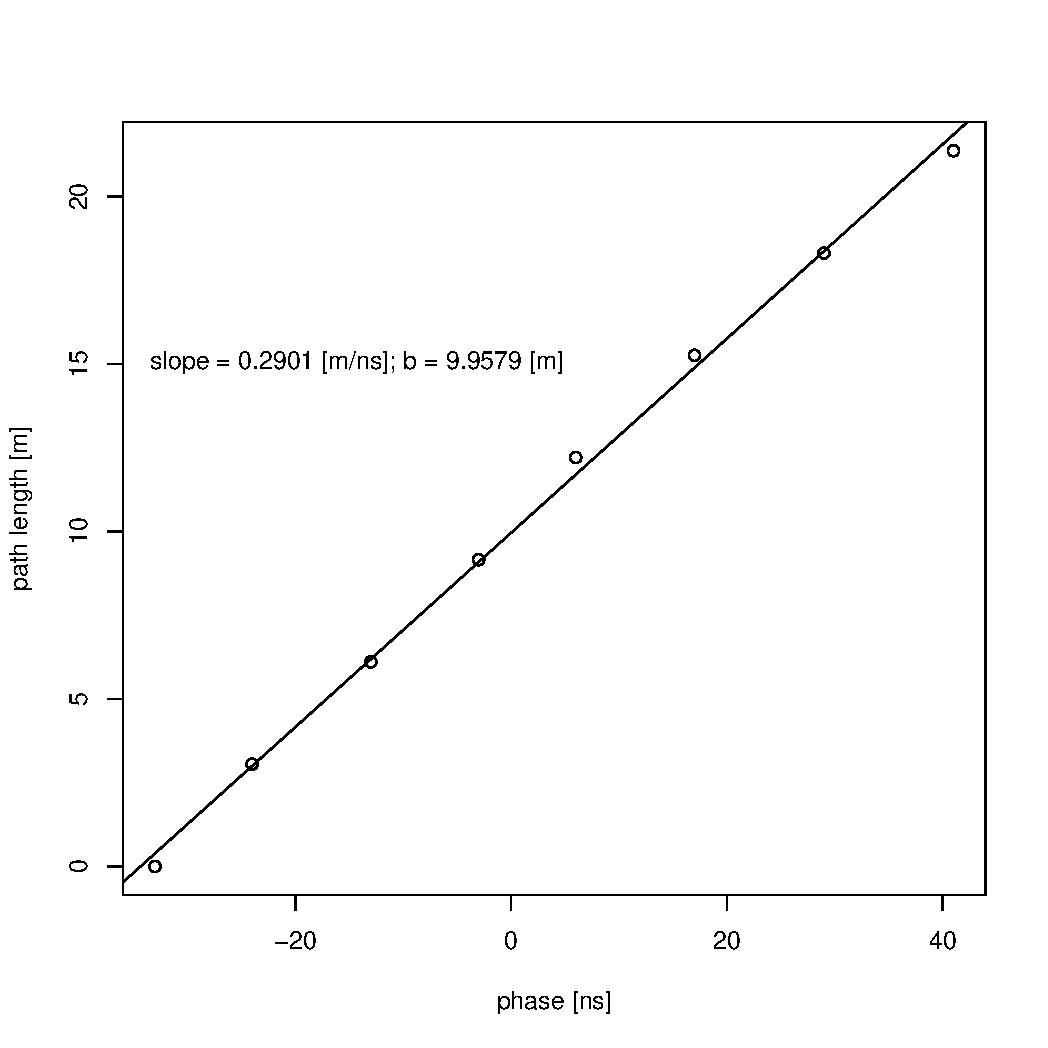
\includegraphics[width=\textwidth]{../images/plot.pdf}
\caption{\label{fig:plot}Plot and fit of sample data for speed of light experiment}
\end{figure}

It is sadly difficult to find fitting software that allows fits to points with error and returns errors on the fitted parameters, slope and $y$-intercept in this case.  In addition to fitting a line to your data, try calculating the slope based on two (widely spaced) points and compare the value for the speed of light you get using the two techniques.  For the simple slope calculation, find the error on the velocity by propagating the estimated errors on $\Delta d^\prime$ and $\Delta t^\prime$.  In your writeup, compare your two values and the world average value in light of this estimated error.

\end{document}
